\chapter{Architecture : site internet}

L'interface du projet est donc un site internet permettant de choisir les destinations de départ et par la suite de gérer les mobilités (partie administrative, gestion des notes, etc).
\bigbreak
Étant donné que deux types d'utilisateurs peuvent accéder au site internet et que ces deux types d'utilisateur n'ont pas la possibilité d'exécuter les mêmes actions; les pages sur lesquels ils naviguerons seront différentes.
\bigbreak
Nous allons vous présenter les différentes pages du sites internet en précisant, en plus de leur utilité, si il existe une version différente pour les administrateurs et les étudiants. 
\bigbreak


\section{Page d'accueil}

\bigbreak

Lors de leur connexion, les utilisateurs sont dirigés sur la page d'accueil réservée à leur catégorie d'utilisateur. Les étudiants seront dirigés sur une page d'accueil dédié et unique à chacun (cf figure \ref{fig::hps}) alors que les administrateur arriverons sur une page contenant de plus nombreuses fonctionnalités (cf figure \ref{fig::hpa}) .
 
\begin{figure}[H]
	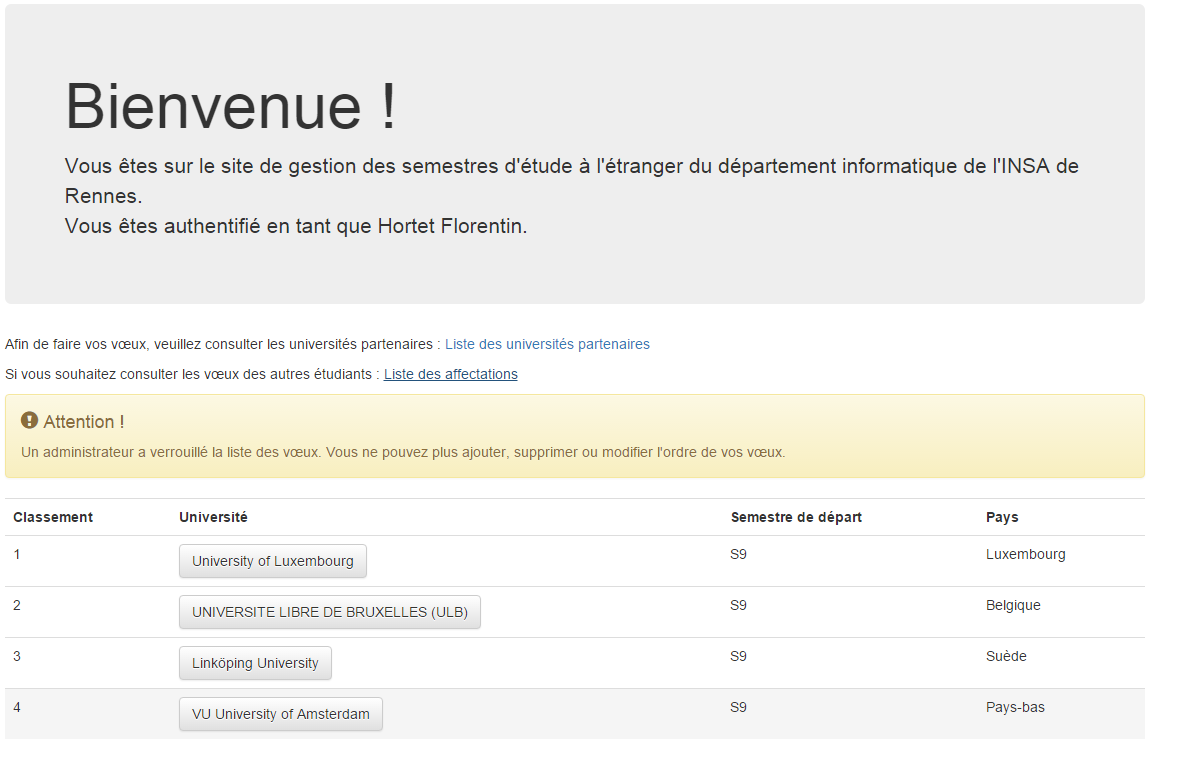
\includegraphics[scale=0.35]{images/HPS.png}
	\caption{Page d'accueil (Étudiant)}
	\label{fig::hps}
\end{figure}

\bigbreak

Comme on peut le voir sur la figure \ref{fig::hps} ci-dessus, lorsque l'élève arrive sur ça page d'accueil, il peut voir la liste des vœux qu'il à fait dans l'ordre de priorité qu'il à choisi. Ici, on peut lire qu'un administrateur a verrouiller les vœux et que l'élève ne peut donc plus modifier ses vœux. Lorsque le choix des vœux n'est pas bloqué par un administrateur, certains boutons supplémentaires apparaissent pour l'élève: un bouton a droite de chacun de ses vœux pour modifier l'ordre des vœux et un pour supprimer un vœux.

\bigbreak

L'étudiant a aussi accès à la liste des universités (cf figure \ref{fig::lus}) ou il pourra faire ses vœux et à une page résumant l'ensemble des vœux des étudiant (cf figure ??)

\begin{figure}[H]
	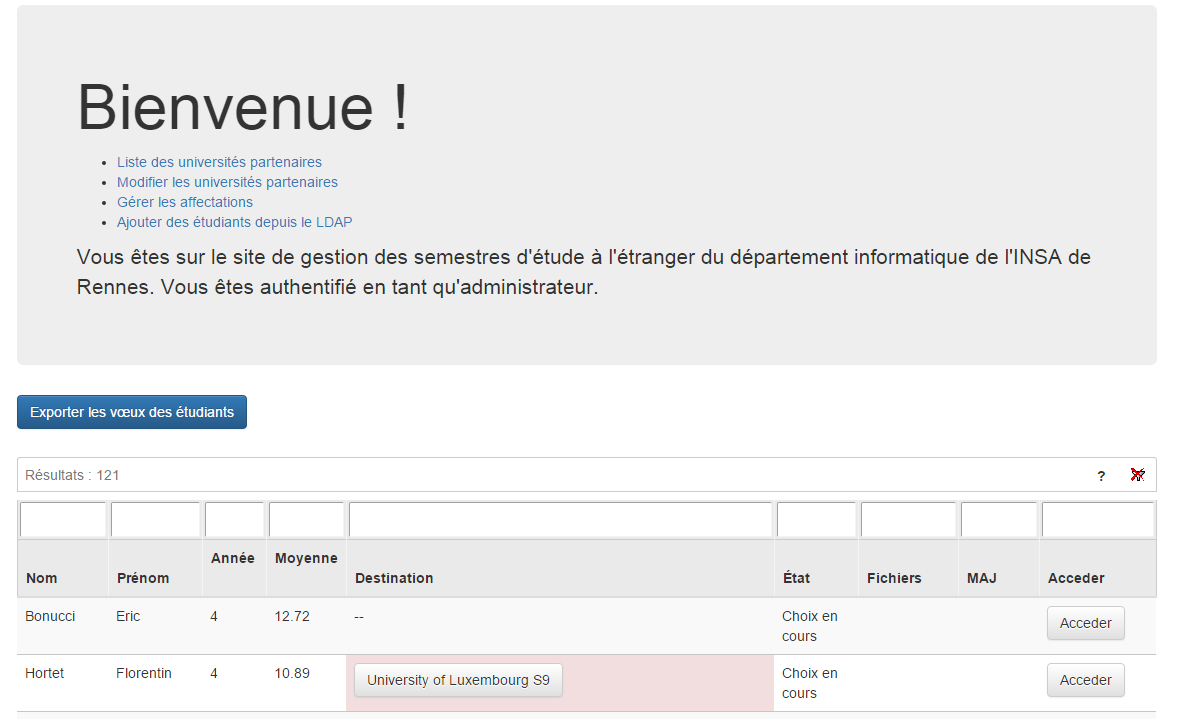
\includegraphics[scale=0.35]{images/HPA.png}
	\caption{Page d'accueil (Administrateur)}
	\label{fig::hpa}
\end{figure}

\bigbreak

L'élément principal de la page d'accueil administrateur est un tableau récapitulatif des élèves regroupant diverses informations sur ces derniers comme leur nom, leur année, leur moyenne leur destination, l'état de l'élève (si il est en train de faire ses choix, si son choix est définitif, si il est partit, etc) ainsi qu'un bouton permettant d'accéder à la page de l'étudiant en mode administrateur (cf figure \ref{fig::pea}).

\bigbreak

En haut de la page, plusieurs liens sont présent:
\begin{itemize}
	\item "Liste des universités partenaires" : permet l'accès à la liste des universités (cf figure \ref{fig::lua});
	\item "Modifier les universités partenaires" : permet d'ajouter de nouvelles universités et de modifier les informations relatives aux universités déjà présentes dans la liste (cf figure ??);
	\item "Gerer les affectations" : permet d'afficher la page de gestion des affectations (cf figure ??);
	\item "ajouter des étudiants depuis le LDAP" : permet d'accéder à la page d'ajout des étudiants dans la base de donnée (cf figure ??);

\end{itemize} 

\bigbreak

\begin{figure}[H]
	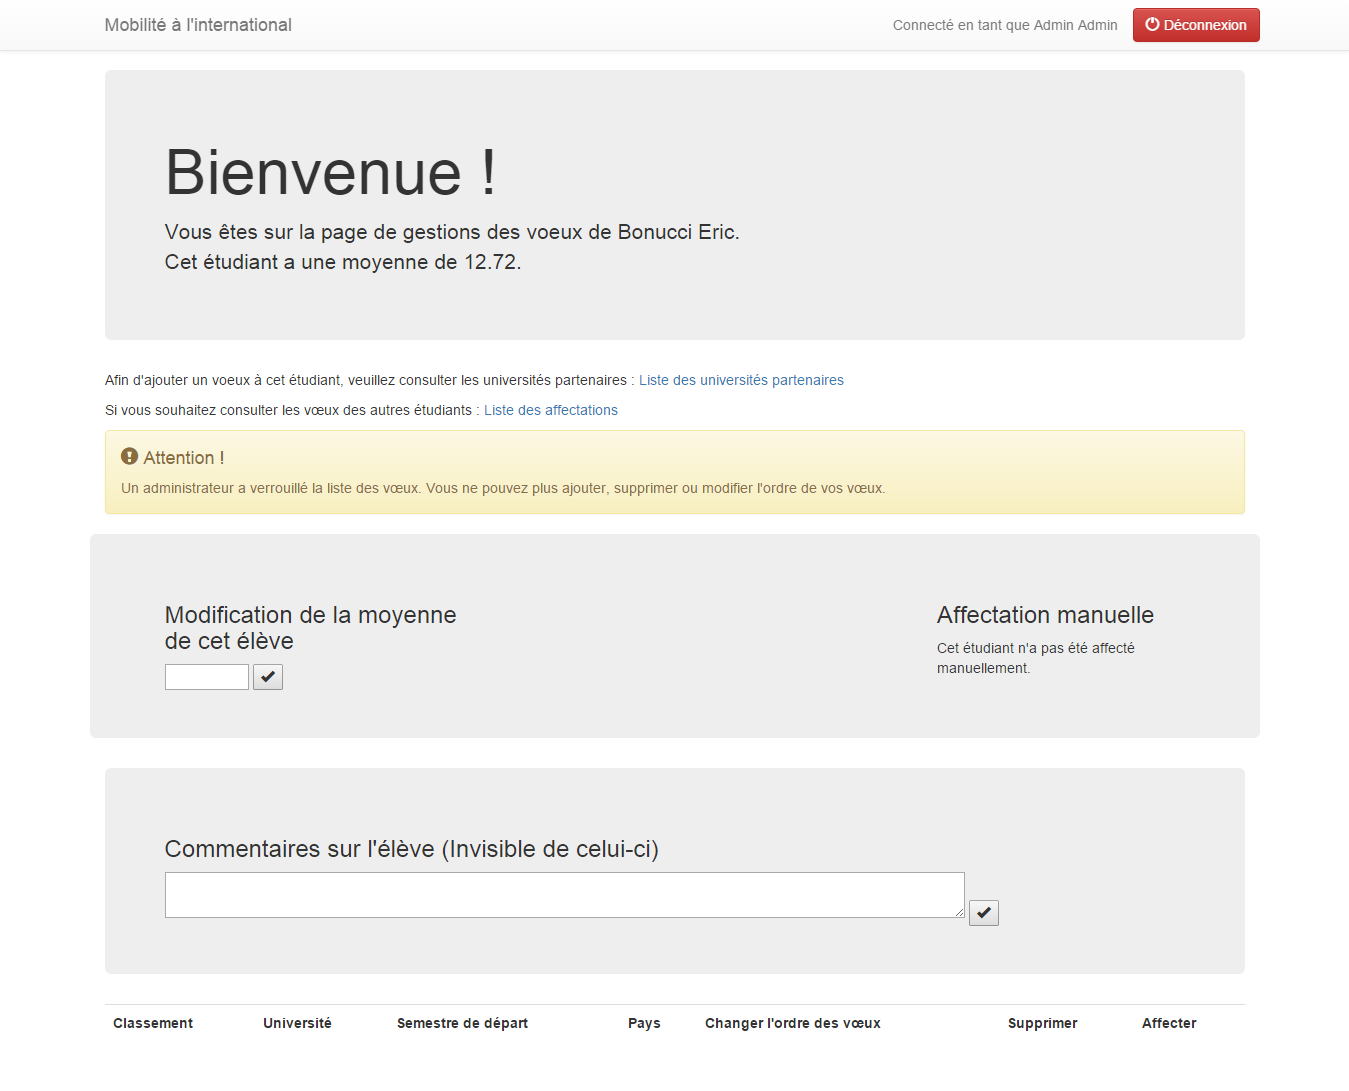
\includegraphics[scale=0.35]{images/PEA.png}
	\caption{Page étudiant (Administrateur)}
	\label{fig::pea}
\end{figure}

En se rendant sur cette page, l'administrateur peut effectuer plusieurs actions sur l'élève. Il est possible de modifier la moyenne de l'étudiant, de l'affecter manuellement et il est possible de laisser un commentaire sur l'élève qui ne sera visible que par les autres administrateurs du département.

\newpage
\section{Liste Université}

\bigbreak

\begin{figure}[H]
	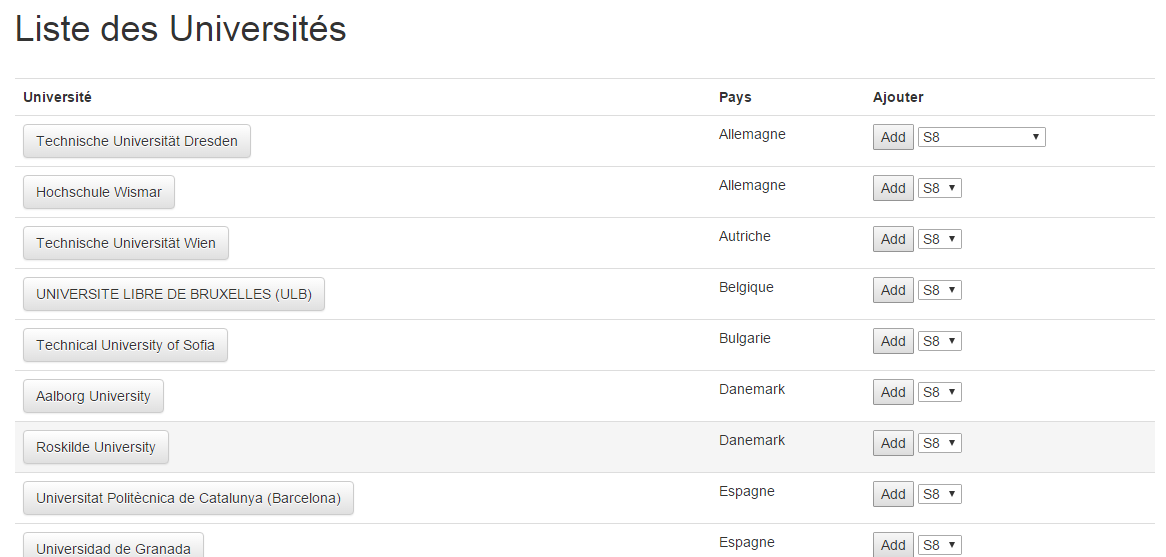
\includegraphics[scale=0.35]{images/LUS.png}
	\caption{Liste des universités (Étudiant)}
	\label{fig::lus}
\end{figure}

Sur cette page, l'étudiant peut voir toutes les universités disponible pour sa mobilité. C'est sur cette page qu'il peut ajouter un vœux. Pour cela, il lui suffit d'indiquer le semestre qu'il souhaite faire à l'étranger (ou bien d'indiquer qu'il s'agit d'un double diplôme si cette option est disponible) et de cliquer sur "ADD" pour l'ajouter à la liste des vœux.

\bigbreak

Dans le cas ou la phase d'ajout de vœux est terminée, effectuer un "ADD" ne fera rien.

\bigbreak

En cliquant sur une université, l'étudiant est redirigé vers la fiche résumé de l'université en question.

\begin{figure}[H]
	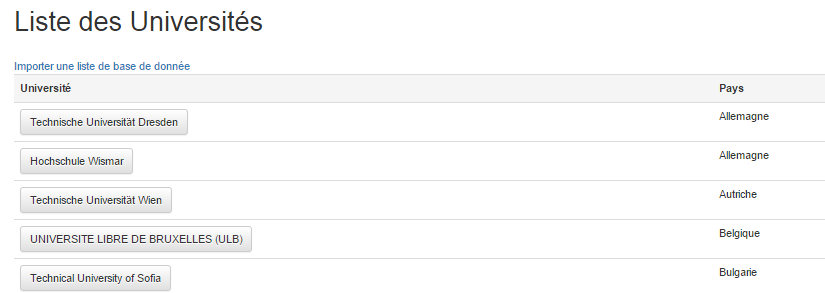
\includegraphics[scale=0.7]{images/LUA.png}
	\caption{Liste des universités  (Administrateur)}
	\label{fig::lua}
\end{figure}

Cette page en version administrateur est la même qu'en version étudiante mais permet, en cliquant sur le lien en haut de la page, d'aller sur la page d'ajout d'universités (cf figure ??). 